\documentclass{article}
\usepackage{graphicx}
\usepackage{fontspec}
\setmainfont{Arial}
\setlength{\parindent}{0pt}
\begin{document}
\section{Users can save money}

Situation now:
\begin{itemize}
\item translate a document to 10 languages
\item each translation costs 1.000€
\item \textbf{cost: 10.000€}
\end{itemize}

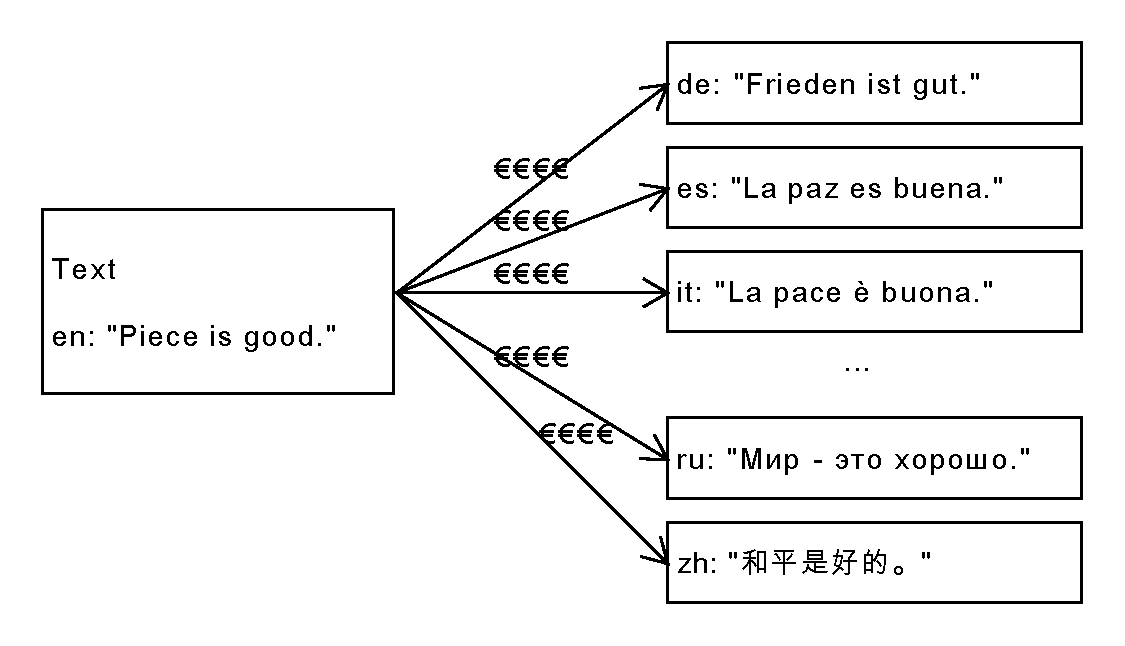
\includegraphics[scale=0.4]{dia/user-view-current-world.pdf}

Goal:
\begin{itemize}
\item encode the document
\item generate 10 language versions
\item encoding costs 2.000€
\item generation doesn't cost anything
\item \textbf{cost: 2.000€}
\end{itemize}

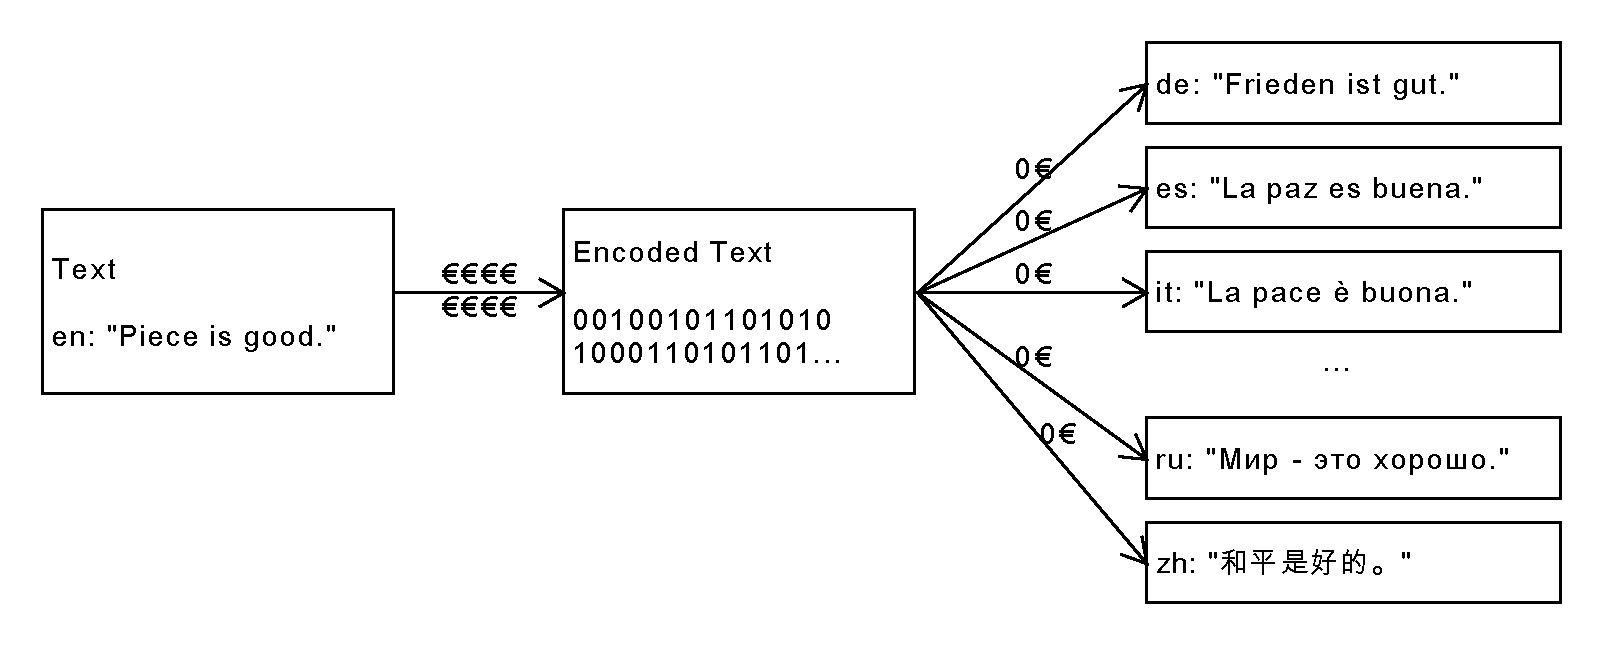
\includegraphics[scale=0.4]{dia/user-view-tokimani.pdf}

Saving: \textbf{8.000€}

\subsection{Some facts about costs}
TODO: how much is spent on translation in the year 2019

TODO: 1.000€ is the cost to translate a document of: 

TODO: in Branchenkennz: xx precent translate to more than k languages.

\section{How}

Existing attempts: full automation

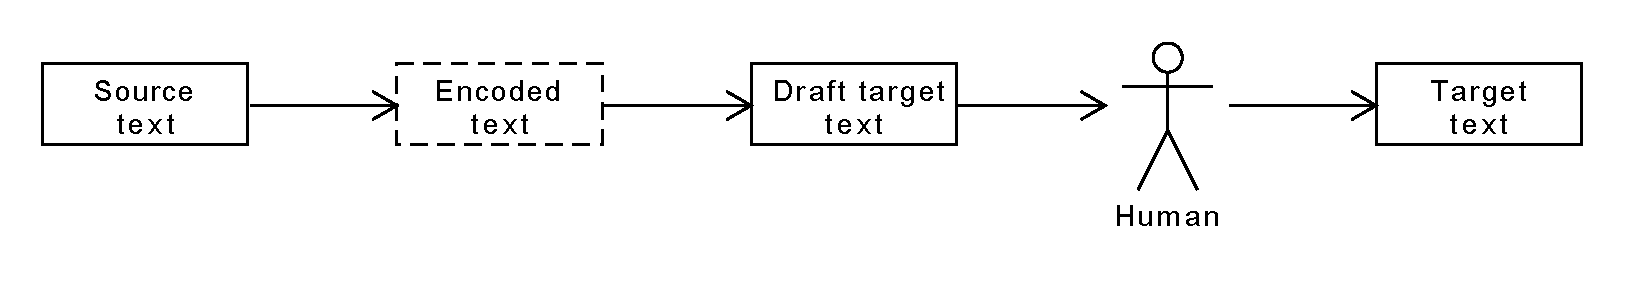
\includegraphics[scale=0.5]{dia/how-current-world.pdf}

Our approach: human in the loop

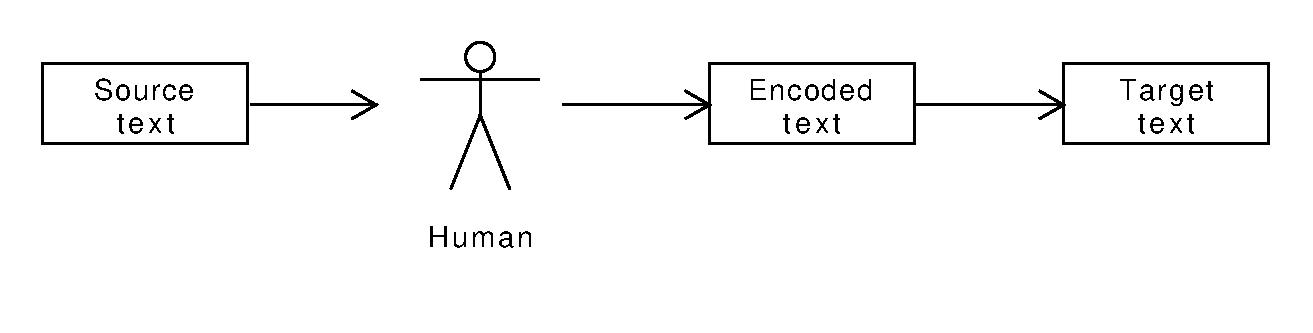
\includegraphics[scale=0.5]{dia/how-tokimani.pdf}

The difference:
\begin{itemize}
\item encoding is made by a human
\item encoded text is human-friendly (for a trained human)
\end{itemize}

\subsection{Why it doesn't exist already}

My hypothesis is: the step "source text to encoded text" can't be automated.

\subsubsection{Fall 1: research}

\begin{itemize}
\item Business has an idea "one source to many targets", likely with the word "automatically".
\item Business ask an university for joint work.
\item Our approach brings nothing scientific new. It leads to no papers. No papers means the end of an academic carier.
\item A researcher subconciously discards our approach even before it comes into mind.
\end{itemize}

\end{document}
